
\section{Indledende designovervejelser}\label{sec:designdatabase}

Til projektet er der udviklet en database som står for at gemme alle brugerdata, herunder en brugers pools samt alle sensordata der foretages derpå.

Den endelige database er udviklet med entity frameworket, med en model first tilgang. Dette er valgt efter mange overvejelser og flere forsøg med forskellige udviklingsmetoder. Dette er beskrevet i detaljer i projekt dokumentationen. \todo{reference til dokumentationen}. I de nedenstående afsnit beskrives designet og implementering af både databasen og data access laget. Måden dette er beskrevet på, vil tage udgangspunkt i to primlre user stories. Den omfattende resterende funktionalitet er beskrevet i projektets dokumentation \todo{reference til doku}

Databasen og DAL har gennemgået 3 udviklingsfaser, første iteration med User, derefter Pool og til sodst Data.

Der er følgene ting i data access laget \todo{vis noget klasse halløj med interfaces}
\subsection{Udvalgte User Story}

Med udgangspunkt i \gls{moscow} analysen blev det første udkast til databasen lavet. Meningen var at opfylde punkterne: 

\begin{itemize}
	\item \textit{"Som bruger vil jeg kunne oprette mig i systemet for at få adgang til systemet"}
	\item \textit{"Som bruger vil jeg kune se de seneste sensorværdier for at kunne få et overblik over poolens tilstand"}
\end{itemize}

\subsection{User story - Oprettelse af en bruger i systemet}

med udgangspunkt i projektets domæneanalyse, blev det gjort klart hvilke attributter en bruger af systemet skulle have.

Disse attributter er vist på figur XXXX

\todo{indsæt ERD for User}

tabellen som vises på XXXX oprettes da i databasen gennem EF.

Med en funktionel database er det nu oplagt at begynde på designet af database access laget.

Der ænskes funktionalitet til at tage brugere u af databasen. der udvikles data access lag til dette.

I forbindelse med udarbejdelsen af disse backend funktonaliter, brugtes Test driven development hvor vi identificere en masse tetcases og scenarioer.

\todo{indsæt test shiz m covereage osv}.

Som de blev slrevet blev tilsvarende business logic og funktionalitet designet og implementeret.
Det har hele tiden været vores tanke at dal skulle være nemt at bruge hos klienten. Vi har derfor designet vores løsning med et simppelt interface, ISmartpoolDB \todo{indst klassediagram for dette interface}.

På denne måde er systemet åbent for udvidelse, da der let kan tilføjes nye Access kklasser. På samme måde er deisgnet depandancy inverted.

Af markante ændringer siden starten kan der nævnes:

\begin{itemize}
	\item FullName entiteten fjernes, User får 3 naming properties.
	\item Residence entiteten fjernes, og Pool entitens \textit{Name} property står for indhold af både addresse og navn.
	\item Value constraints fjernes helt da de ikke er nødvendige at have på databasen
	\item PoolDimensions entiteten fjernes, og Pool får en \textit{Volume} property.
	\item MonitorUnit entiteten udgår af fra databasen. Denne har kun været i databasen for at checke på et evt. serienummer.
	\item Persistering af data er blevet smartere, se figur \ref{fig:databaseERD_final_uml}.
\end{itemize}

\begin{figure}[h]
	\centering
	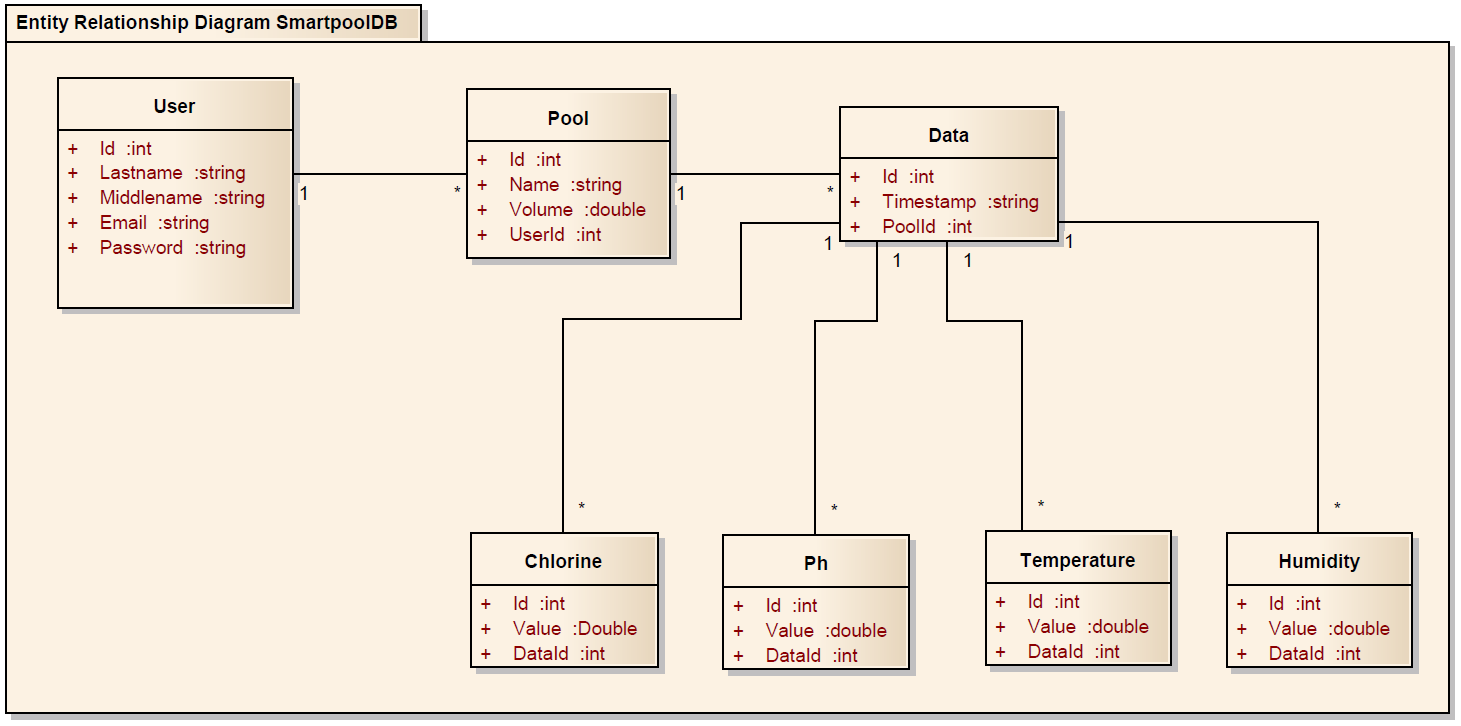
\includegraphics[width=\linewidth]{figs/design/databaseERD_final_uml}
	\caption{Endeligt ER diagram, UML notation}
	\label{fig:databaseERD_final_uml}
\end{figure}

En klient kan kalde sig ind i alt dal's funktionalitet gennem ISmartpoolDB interfcet.

\todo{indsæt noget om den konkrete implmentering - Find de fedeste kodebidder og sæt in med kommentarer}


\subsection{User story - Se sensor værdier}

Eftersom funktionalitet til oprettelse af bruger og Pools blev laveet, var  det tid til at gå i gang med sensordata ting.

Dette var 3 fase, og vi havde derfor en fuldt fungerende User og Pool. Måden sensordata persisteres på i databasen skiller sig en smule ud fra måden hvor fx en USer eller en pool gøres. \todo{indsæt ER diagram for data og dtatyper}. Som det kan ses på figur XXXX indeholder databasen 4 typer af sensor målinger, samt en Data entitet. Is tedet for at hver enkel sensortype entitet indeholder et timestamp, har vi valgt at ligge timestampet på Dataentiteten. Dett gøres for at det samme timestamp ikke skal ligge på flere data - undgå redundant data.  Samtidig hvis man gerne vil have ex luftfugtighed i samme tidsrum som klor level, er det vigtgt at målingernes timestamp er den samme.

Der er lavet en dataAccess klasse til at lave data wueries og skrivninger til databasen. Se klassediagra \todo{indsæt her}

Igen brugtes test driven development til dette, hvor koden blev skrevet til testene.  \todo{indæt mere test bragging}.

Der er til dataaccess lavet it interface som initialiseret af SmartpoolDB.

Måden hvorpå der trækkes data ud af databasen er ved hjælp af LINQ ueries. \todo{skriv lidt om LINQ qureis og hvordan man bruger dem}. Brugen heraf er skrevet i detaljer idokumenttionen.

Her på XXXX vises hvordan DALS getter metoder bruges af en klient.\ todo{indsæt kodeudsnit fra windserver}